\documentclass[../Article_Model_Parameters.tex]{subfiles}
\graphicspath{{\subfix{../Figures/}}}
\begin{document}
	
	\label{CH: Results}

    The parameter estimation problem was solved by fitting the process model to the dataset given in the Table \ref{tab: Yield_data}. Each time-series was fitted to the model separately. As a result of fitting, the following parameters were obtained:

    \begin{itemize}
        \item Partition coefficient:\qquad\quad\qquad$k_m$
        \item Internal Diffusion coefficient: \quad$D_i$
        \item Axial Diffusion coefficient: \qquad$D_e^M$
        \item Saturation concentration: \quad\qquad$C_{sat}$
        \item Standard Deviation: \qquad\qquad\quad$\sigma$
    \end{itemize}

    Moreover, the initial state estimation was performed together with parameter estimation. The concentration of solute in the solid phase is assumed to be constant and uniformly distributed. On the other hand, the solute concentration in the fluid phase should not follow the same assumption as the solid phase. During the preparation period the solute diffuses to the fluid phase in contact with the solid particles. Later, the solute in the fluid phase is partially moved along the extractor (if the pressure increase in the system, the pump cause the movement of the fluid, even if the outlet valve is closed). As a result, the distribution of solute mass in the fluid phase is assumed to not be uniform. Some conclusions can be drawn from the analysis of the initial part of each yield curve. It can be noticed that each curve at the beginning has a curvature, which is not linear. In a general sense, it can be said that a quadratic function could approximate the initial part of each extraction curve. A function that, after integration, gives a quadratic-like result is a straight line. Based on that observation, the solute concentration in the fluid phase is assumed to be linearly distributed. The solute concentration is assumed to be zero at the outlet and reach the maximum at the beginning of the fixed bed. The details on the calculation are given in appendix \ref{CH: IC_BC}. The linear distribution can be defined if the total mass of solute $m_{total}$ and partition coefficient $\tau$ are know.
    
    Due to initial state estimation, two additional parameters are fitted.

    \begin{itemize}
        \item Total mass of solute: \qquad\qquad\quad$m_{total}$
        \item Partition coefficient: \qquad\qquad\quad$\tau$
    \end{itemize}

	To ensure that parameters found by the optimizer do not reach unrealistic values, an additional set of inequality constraints is introduced. The lower and upper bounds for each parameter are given in Table \ref{tab:Constraints}. To ensure that the solution is a global solution multiple initial points have been tested but presented results come from the initial guess given also in Table \ref{tab:Constraints}.

	\begin{table}[!h]
		\centering
		\adjustbox{max width=\columnwidth}{%
		\begin{tabular}{ lccccccc }
			\hline 
			Parameter		&$k_m$[-] 	& $D_i$[m/s$^2$] 	& $D_e^M$[m/s$^2$]	& $C_{sat}$ [kg/m$^3$] 	& $m_{total}$[g]	& $\tau$[-] 	& $\sigma$[-] \\  \hline
			Lower bound		&0	  		& 0 	  			& 0 				&	0					& 80 		 		& 0 	   		& 0 \\ 
			Upper bound		&1 			& $+\infty$ 		& $+\infty$			&	$+\infty$			& 150 				& 1 			& $+\infty$ \\ 
			Initial guess	&1	  		& 3 	  			& 1 				&	3					& 80 		 		& 0.65 	   		& 0.1 \\  \hline
		\end{tabular} }
	\caption{Constraints and initial guess of the parameter estimation problem}
	\label{tab:Constraints}
	\end{table}

%	The parameter estimation problem requires an initial guess as an input to an optimization problem. To ensure that the solution is a global solution multiple initial points have been tested. The initial guesses for the parameter estimation problem are given in Table \ref{tab:InitialGuess}
	
%	\begin{table}[!h]
%		\centering
%		\adjustbox{max width=\columnwidth}{%
%		\begin{tabular}{ lcccccc } 
%			\hline
%			Parameter		&$k_m$ 	& $D_i$ 	& $D_e^M$ 	& $m_{total}$	& $\tau$ 	& $\sigma$ \\  \hline
%			Initial guess	&1	  	& 3 	  	& 1 		& 77 		 	& 0.65 	   	& 0.1 \\  \hline
%		\end{tabular} }
%		\caption{Constraints of the parameter estimation problem}
%		\label{tab:InitialGuess}
%	\end{table}
	
	Figure \ref{fig: estimation_results} show yield curves for each of experiments. The blue dots indicate the data point obtained as a measurement from the laboratory experiments. The black curve represents the yield curve obtained from the initial guess of the parameters. The blue curve correspond to yield curve obtained as a solution of the optimization problem. The curves on the left hand-side of the Figure \ref{fig: estimation_results}, are the cumulative yield curves, which represents the cumulative amount of the oil collected during each experiment. The plots on the right hand-side, represent the derivative of the cumulative yield curves. As explained in the chapter \ref{CH: Parameter_estimation}, the derivatives of the cumulative measurements are independent on the previous measurement and should be used for the parameter estimation.

	\begin{table}[!h]
		\centering
		\adjustbox{max width=\columnwidth}{%
			\csvautobooktabular{Figures/Results_estimation/estimation.csv} }
		\caption{Parameter estimation results rounded to fifth decimal place}
		\label{tab: Estimation_results}
	\end{table}

	The results of parameter estimation can be found in Table \ref{tab: Estimation_results} and the concentration profiles, which correspond for the optimized solution for each experiments, are presented on Figure \ref{fig: estimation_results_profiles} in Appendix \ref{CH: Profiles}. As can be noticed, the optimizer found that the partition factor should be as high as possible and moved values of $k_m$ for each experiment to unity, which was chosen as the upper bound.
		
	Values of the internal diffusion coefficients are distinguished for each experiment, which grows as the fluid density increase. The order of magnitude of $D_i$ obtained from the optimization is similar to values found by other researchers. \citet{Reverchon1996} performed the parameter estimation for the extraction process of sage oil from seeds and reported $D_i \approx 6e-13$.
	
	The axial diffusion coefficient obtained from the optimizer seems to be quite high if compared to the internal diffusion coefficients. Nevertheless, the values of $D_e^M$ have similar order of magnitude as reported in literature, for example \citet{ReisVasco2000}. The relatively high values of the axial diffusion coefficients might be justified by taking into account low values of flow rate used in all the experiments.
	
	The further spifflication of the process model can be introduced based on $C_{sat}$ results. Values of saturation concentrations are at the level of 1e5 which is an internal upper bound of the optimizer used if $+\infty$ indicates the upper bound. This suggest that solvent hasn't reach the saturation concentration and the process model can be simplified by replacing $\gamma(c_f)$ function with unity.
	
	As the total amount of the oil present in the system is unknown, and as such it has been obtained from the optimizer. Given the dataset and the process model, the optimizer found that the best fit is obtained if the total mass of the oil reach a lower bound equal to 80 g. The lower bound was estimated by round up of the biggest value of collected cumulative amount of the extraction product. As the same raw material was used in all experiments, the same initial amount of solute is assumed for all the cases.
	
	As explained above, and in Appendix \ref{CH: IC_BC}, the linear distribution of can be fully determined if the parameter $\tau$ is known. The split ratio for experiments conducted at $40 ^\circ C$ / 300 bar and $50 ^\circ C$ / 300 bar are similar to each other and close to 0.65. The experiments performed at $40 ^\circ C$ / 200 bar and $50 ^\circ C$ / 200 bar have $\tau$ equals to $0.70$ and $0.75$, respectively. 
	
	The noise present in each dataset is quantified by parameter $\sigma$. It can be observed dataset obtained at $40 ^\circ C$ / 200 bar and $50 ^\circ C$ / 200 bar have similar value of $\sigma\approx0.36$. The visual investigation of the datasets obtained at $40 ^\circ C$ / 300 bar and $50 ^\circ C$ / 300 bar allow to explain higher values of $\sigma$ for both dataset. Both datasets have higher deviation of the data points from the simulated curve.
	
	\begin{figure}[!h]
		\centering
		\begin{subfigure}[b]{\columnwidth}
			\centering
			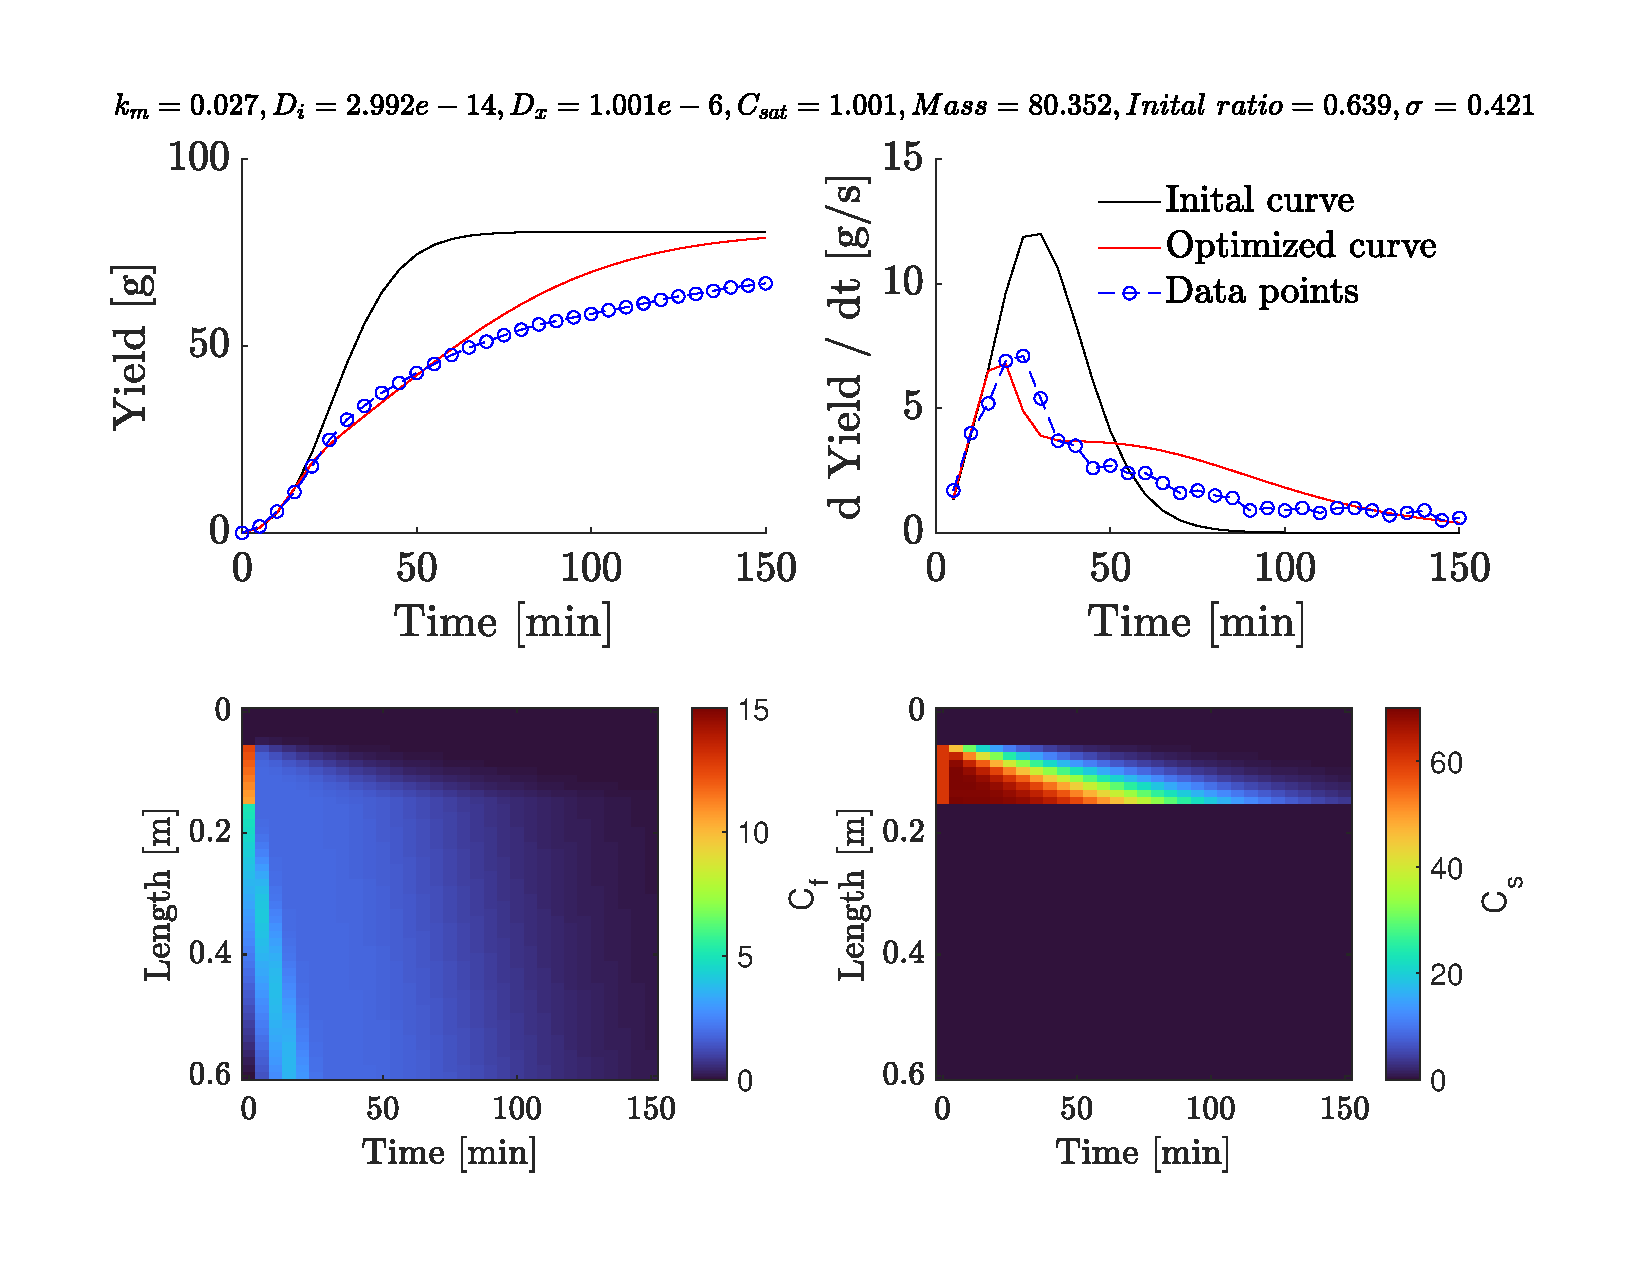
\includegraphics[trim = 2cm 10.5cm 2.5cm 2.02cm,clip,width=\textwidth]{/Results_estimation/Fitting_LUKE_T40_P200.pdf}
			\caption{Experiment at $40^\circ C$ and $200$ bar}
		\end{subfigure}
		\begin{subfigure}[b]{\columnwidth}
			\centering
			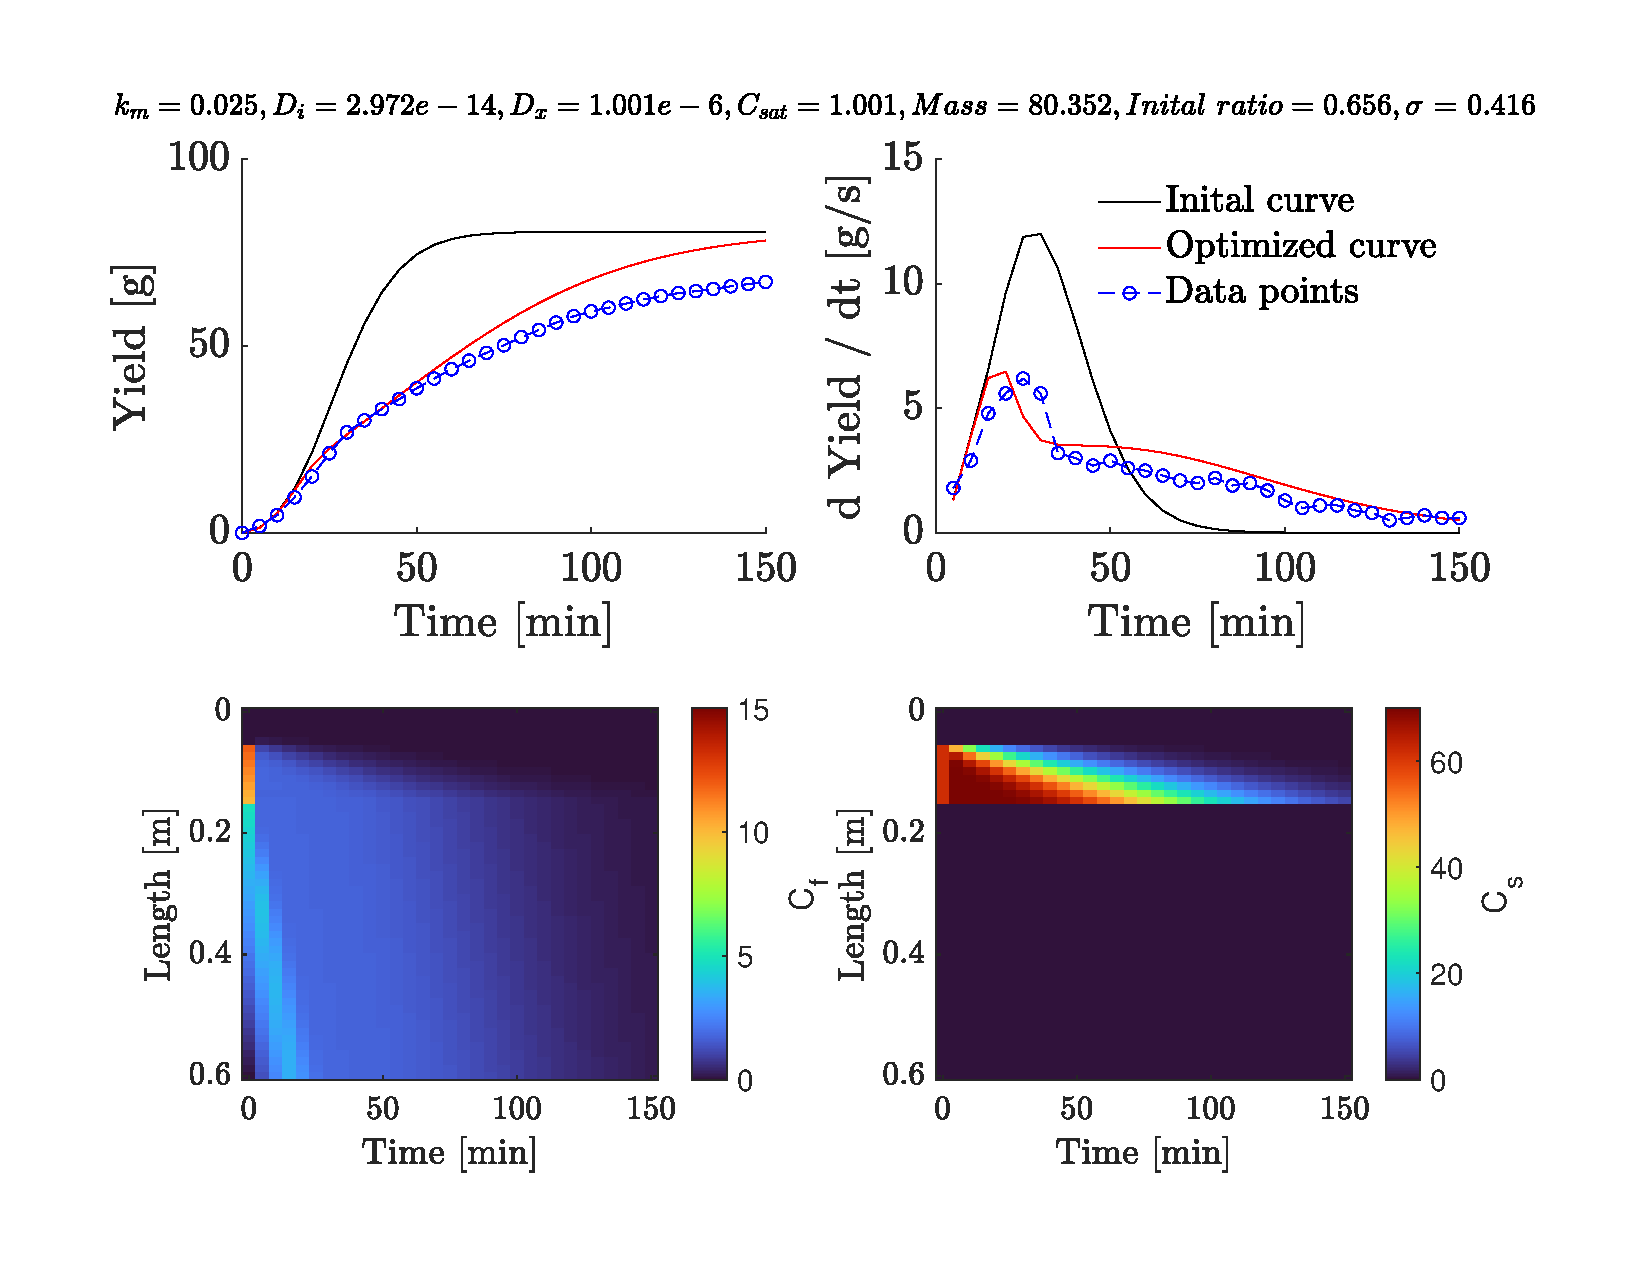
\includegraphics[trim = 2cm 10.5cm 2.5cm 2.02cm,clip,width=\textwidth]{/Results_estimation/Fitting_LUKE_T50_P200.pdf}
			\caption{Experiment at $50^\circ C$ and $200$ bar}
		\end{subfigure}
		\begin{subfigure}[b]{\columnwidth}
			\centering
			\includegraphics[trim = 2cm 10.5cm 2.5cm 2.02cm,clip,width=\textwidth]{/Results_estimation/Fitting_LUKE_T40_P300_org.pdf}
			\caption{Experiment at $40^\circ C$ and $300$ bar}
		\end{subfigure}
		\begin{subfigure}[b]{\columnwidth}
			\centering
			\includegraphics[trim = 2cm 10.5cm 2.5cm 2.02cm,clip,width=\textwidth]{/Results_estimation/Fitting_LUKE_T50_P300_org.pdf}
			\caption{Experiment at $50^\circ C$ and $300$ bar}
		\end{subfigure}
		\caption{Results of parameter fitting, with estimation of the initial state}
		\label{fig: estimation_results}
	\end{figure}

	The results obtained from the parameter estimation are used to develop a generalized process model. The model generalization is performed by introducing correlations which link the estimated parameters and the operating conditions. Since the experiments were performed under varying temperature and pressure, the influence of these variables is taken into account. To simplify the problem, the correlations are written as functions of fluid density rather than temperature and pressure. Since the optimizer found that $k_m$, $m_{total}$ and $C_{sat}$ don't change with the density variations, they are assumed to be constants and not considered further.
		
	The other two parameters ($D_i$ and $D_e^M$) are subject to regression to obtain correlations in terms of density. Figure \ref{fig:Regression} shows the first- and second-order polynomials used to fit $D_i$ and $D_e^M$ as a function of fluid density. 
	
	\begin{figure}[!h]
	\centering
	\begin{subfigure}[b]{\columnwidth}
		\centering
		\includegraphics[trim = 11.7cm 14cm 2.3cm 1cm,clip,width=\textwidth]{/Results_estimation/Trend_Lines_order_1.pdf}
		\caption{First-order polynomial regression of fitted parameters ($D_i$ and $D_e^M$) as a function of fluid density $\rho_f$}
		\label{fig:Regression_1}
	\end{subfigure}
	\begin{subfigure}[b]{\columnwidth}
		\centering
		\includegraphics[trim = 11.7cm 14cm 2.3cm 1cm,clip,width=\textwidth]{/Results_estimation/Trend_Lines_order_2.pdf}
		\caption{Second-order polynomial regression of fitted parameters ($D_i$ and $D_e^M$) as a function of fluid density $\rho_f$}
		\label{fig:Regression_2}
	\end{subfigure}
	\caption{Regression of $D_i$ and $D_e^M$} 
	\label{fig:Regression}
	\end{figure}

	The results of the linear regression applied to $D_i$ and $D_e^M$ are presented in Figure \ref{fig:Regression_1}. It can be observed that the internal diffusion coefficient increases with increasing fluid density, while the axial diffusion coefficient decreases.
	
	The increase in the density of the supercritical fluid can lead to an increase in the solubility of the solute and, consequently, an increase in the concentration gradient. This increased concentration gradient drives the solute to diffuse more rapidly through the matrix of the solid particles, resulting in an increased internal mass transfer coefficient. However, the effect of increased solubility on the internal mass transfer coefficient outweighs the resistance from higher density, resulting in an overall increase in the internal mass transfer coefficient with density. The same behaviour can be observed in Figure \ref{fig: estimation_results}, where plots on the right-hand side exhibit a peak. The higher the peak, the greater the increase in solute concentration in the fluid phase, which can be explained by higher solubility.
	
	The behaviour of the axial diffusion coefficient can be explained through Graham’s Law of Diffusion, which states that the rate of diffusion of a molecule is inversely proportional to the square root of its density under given conditions of temperature and pressure. This means that denser media slow down the axial diffusion rate of molecules. 
	
	{\color{red}IDEAL I SHOULD SUPPORT THIS EXPLANATION WITH SOME REFERENCES}
	
	Figure \ref{fig:Regression_2} show the result of fitting a second-order polynomial in density space. It can be observed that the fit obtained from quadratic functions seems to be represent both dataset better. 
	
	The experimental procedure and the used device can influence the values of $\tau$ and $\sigma$. Therefore, seeking a general expression for the initial state that is solely a function of operating conditions may not be sufficient to fully describe the relationship between these parameters. However, if first- and second-order regressions are applied to $\tau$ and $\sigma$, some general conclusions about the trend can be drawn. The results of the regression applied to $\tau$ and $\sigma$ are presented in Figure \ref{fig:Regression_tau_simga}.
	
	\begin{figure}[!h]
		\centering
		\begin{subfigure}[b]{\columnwidth}
			\centering
			\includegraphics[trim = 18.8cm 8cm 2.5cm 7.6cm,clip,width=0.49\textwidth]{/Results_estimation/Trend_Lines_order_1.pdf}
			\includegraphics[trim = 4cm 2cm 17.5cm 13.6cm,clip,width=0.49\textwidth]{/Results_estimation/Trend_Lines_order_1.pdf}
			\caption{First order polynomial regression of fitted parameters ($\tau$ and $\sigma$) as a function of fluid density $\rho_f$}
			\label{fig:Regression_3}
		\end{subfigure}
		\begin{subfigure}[b]{\columnwidth}
			\centering
			\includegraphics[trim = 18.8cm 8cm 2.5cm 7.6cm,clip,width=0.49\textwidth]{/Results_estimation/Trend_Lines_order_2.pdf}
			\includegraphics[trim = 4cm 2cm 17.5cm 13.6cm,clip,width=0.49\textwidth]{/Results_estimation/Trend_Lines_order_2.pdf}
			\caption{Second order polynomial regression of fitted parameters ($\tau$ and $\sigma$) as a function of fluid density $\rho_f$}
			\label{fig:Regression_4}
		\end{subfigure}
		\caption{Regression of $\tau$ and $\sigma$} 
		\label{fig:Regression_tau_simga}
	\end{figure}

	As can be seen from Figure \ref{fig:Regression_tau_simga} , the $\tau$ seems to decrease as the fluid density increase. The standard deviation increases as the fluid density increase. As mentioned above, these results should be used with caution due to uninvestigated influence of the equipment on the extraction results.
	
	To prove that the obtained solution is a global solution, the parameter estimation problem was run from multiple initial conditions. The Appendix \ref{CH: Profiles_2}, contain a solution of the optimization solution and corresponding figures.
	
\end{document}